%  A simple AAU report template.
%  2015-05-08 v. 1.2.0
%  Copyright 2010-2015 by Jesper Kjær Nielsen <jkn@es.aau.dk>
%
%  This is free software: you can redistribute it and/or modify
%  it under the terms of the GNU General Public License as published by
%  the Free Software Foundation, either version 3 of the License, or
%  (at your option) any later version.
%
%  This is distributed in the hope that it will be useful,
%  but WITHOUT ANY WARRANTY; without even the implied warranty of
%  MERCHANTABILITY or FITNESS FOR A PARTICULAR PURPOSE.  See the
%  GNU General Public License for more details.
%
%  You can find the GNU General Public License at <http://www.gnu.org/licenses/>.
%
%  A simple AAU report template.
%  2015-05-08 v. 1.2.0
%  Copyright 2010-2015 by Jesper Kjær Nielsen <jkn@es.aau.dk>
%
%  This is free software: you can redistribute it and/or modify
%  it under the terms of the GNU General Public License as published by
%  the Free Software Foundation, either version 3 of the License, or
%  (at your option) any later version.
%
%  This is distributed in the hope that it will be useful,
%  but WITHOUT ANY WARRANTY; without even the implied warranty of
%  MERCHANTABILITY or FITNESS FOR A PARTICULAR PURPOSE.  See the
%  GNU General Public License for more details.
%
%  You can find the GNU General Public License at <http://www.gnu.org/licenses/>.
%
\documentclass[12pt,twoside,a4paper,openright]{report}
%%%%%%%%%%%%%%%%%%%%%%%%%%%%%%%%%%%%%%%%%%%%%%%%
% Language, Encoding and Fonts
% http://en.wikibooks.org/wiki/LaTeX/Internationalization
%%%%%%%%%%%%%%%%%%%%%%%%%%%%%%%%%%%%%%%%%%%%%%%%
% Select encoding of your inputs. Depends on
% your operating system and its default input
% encoding. Typically, you should use
%   Linux  : utf8 (most modern Linux distributions)
%            latin1 
%   Windows: ansinew
%            latin1 (works in most cases)
%   Mac    : applemac
% Notice that you can manually change the input
% encoding of your files by selecting "save as"
% an select the desired input encoding. 
\usepackage[utf8]{inputenc}
% Make latex understand and use the typographic
% rules of the language used in the document.
\usepackage[danish,english]{babel}
% Use the palatino font
\usepackage[sc]{mathpazo}
\linespread{1.05}         % Palatino needs more leading (space between lines)
% Choose the font encoding
\usepackage[T1]{fontenc}
%%%%%%%%%%%%%%%%%%%%%%%%%%%%%%%%%%%%%%%%%%%%%%%%
% Graphics and Tables
% http://en.wikibooks.org/wiki/LaTeX/Importing_Graphics
% http://en.wikibooks.org/wiki/LaTeX/Tables
% http://en.wikibooks.org/wiki/LaTeX/Colors
%%%%%%%%%%%%%%%%%%%%%%%%%%%%%%%%%%%%%%%%%%%%%%%%
% load a colour package
\usepackage{xcolor}
\definecolor{aaublue}{RGB}{33,26,82}% dark blue
% The standard graphics inclusion package
\usepackage{graphicx}
% Set up how figure and table captions are displayed
\usepackage{caption}
\captionsetup{%
  font=footnotesize,% set font size to footnotesize
  labelfont=bf % bold label (e.g., Figure 3.2) font
}
% Make the standard latex tables look so much better
\usepackage{array,booktabs}
% Enable the use of frames around, e.g., theorems
% The framed package is used in the example environment
\usepackage{framed}

%%%%%%%%%%%%%%%%%%%%%%%%%%%%%%%%%%%%%%%%%%%%%%%%
% Mathematics
% http://en.wikibooks.org/wiki/LaTeX/Mathematics
%%%%%%%%%%%%%%%%%%%%%%%%%%%%%%%%%%%%%%%%%%%%%%%%
% Defines new environments such as equation,
% align and split 
\usepackage{amsmath}
% Adds new math symbols
\usepackage{amssymb}
% Use theorems in your document
% The ntheorem package is also used for the example environment
% When using thmmarks, amsmath must be an option as well. Otherwise \eqref doesn't work anymore.
\usepackage[framed,amsmath,thmmarks]{ntheorem}

%%%%%%%%%%%%%%%%%%%%%%%%%%%%%%%%%%%%%%%%%%%%%%%%
% Page Layout
% http://en.wikibooks.org/wiki/LaTeX/Page_Layout
%%%%%%%%%%%%%%%%%%%%%%%%%%%%%%%%%%%%%%%%%%%%%%%%
% Change margins, papersize, etc of the document
\usepackage[
  inner=28mm,% left margin on an odd page
  outer=41mm,% right margin on an odd page
  ]{geometry}
% Modify how \chapter, \section, etc. look
% The titlesec package is very configureable
\usepackage{titlesec}
\titleformat{\chapter}
{\filcenter\normalfont\Large\bfseries}
{\chaptertitlename~\thechapter} {0.5em} {}
\titleformat*{\section}{\normalfont\Large\bfseries}
\titleformat*{\subsection}{\normalfont\large\bfseries}
\titleformat*{\subsubsection}{\normalfont\normalsize\bfseries}
%\titleformat*{\paragraph}{\normalfont\normalsize\bfseries}
%\titleformat*{\subparagraph}{\normalfont\normalsize\bfseries}

% Clear empty pages between chapters
\let\origdoublepage\cleardoublepage
\newcommand{\clearemptydoublepage}{%
  \clearpage
  {\pagestyle{empty}\origdoublepage}%
}
\let\cleardoublepage\clearemptydoublepage

% Change the headers and footers
\usepackage{fancyhdr}
\pagestyle{fancy}
\fancyhf{} %delete everything
\renewcommand{\headrulewidth}{0pt} %remove the horizontal line in the header
\fancyhead[RE]{\small\nouppercase\leftmark} %even page - chapter title
\fancyhead[LO]{\small\nouppercase\rightmark} %uneven page - section title
\fancyhead[LE,RO]{\thepage} %page number on all pages
% Do not stretch the content of a page. Instead,
% insert white space at the bottom of the page
\raggedbottom
% Enable arithmetics with length. Useful when
% typesetting the layout.
\usepackage{calc}

%%%%%%%%%%%%%%%%%%%%%%%%%%%%%%%%%%%%%%%%%%%%%%%%
% Bibliography
% http://en.wikibooks.org/wiki/LaTeX/Bibliography_Management
%%%%%%%%%%%%%%%%%%%%%%%%%%%%%%%%%%%%%%%%%%%%%%%%
\usepackage[backend=bibtex,
  bibencoding=utf8
  ]{biblatex}
\addbibresource{bib/mybib}

%%%%%%%%%%%%%%%%%%%%%%%%%%%%%%%%%%%%%%%%%%%%%%%%
% Misc
%%%%%%%%%%%%%%%%%%%%%%%%%%%%%%%%%%%%%%%%%%%%%%%%
% Add bibliography and index to the table of
% contents
\usepackage[nottoc]{tocbibind}
% Add the command \pageref{LastPage} which refers to the
% page number of the last page
\usepackage{lastpage}
% Add todo notes in the margin of the document
\usepackage[
%  disable, %turn off todonotes
  colorinlistoftodos, %enable a coloured square in the list of todos
  textwidth=\marginparwidth, %set the width of the todonotes
  textsize=scriptsize, %size of the text in the todonotes
  ]{todonotes}

%%%%%%%%%%%%%%%%%%%%%%%%%%%%%%%%%%%%%%%%%%%%%%%%
% Hyperlinks
% http://en.wikibooks.org/wiki/LaTeX/Hyperlinks
%%%%%%%%%%%%%%%%%%%%%%%%%%%%%%%%%%%%%%%%%%%%%%%%
% Enable hyperlinks and insert info into the pdf
% file. Hypperref should be loaded as one of the 
% last packages
\usepackage{hyperref}
\hypersetup{%
	pdfpagelabels=true,%
	plainpages=false,%
	pdfauthor={Author(s)},%
	pdftitle={Title},%
	pdfsubject={Subject},%
	bookmarksnumbered=true,%
	colorlinks=false,%
	citecolor=black,%
	filecolor=black,%
	linkcolor=black,% you should probably change this to black before printing
	urlcolor=black,%
	pdfstartview=FitH%
}% package inclusion and set up of the document
% see, e.g., http://en.wikibooks.org/wiki/LaTeX/Formatting#Hyphenation
% for more information on word hyphenation
\hyphenation{ex-am-ple hy-phen-a-tion short}
\hyphenation{long la-tex}
% 
%  A simple AAU report template.
%  2015-05-08 v. 1.2.0
%  Copyright 2010-2015 by Jesper Kjær Nielsen <jkn@es.aau.dk>
%
%  This is free software: you can redistribute it and/or modify
%  it under the terms of the GNU General Public License as published by
%  the Free Software Foundation, either version 3 of the License, or
%  (at your option) any later version.
%
%  This is distributed in the hope that it will be useful,
%  but WITHOUT ANY WARRANTY; without even the implied warranty of
%  MERCHANTABILITY or FITNESS FOR A PARTICULAR PURPOSE.  See the
%  GNU General Public License for more details.
%
%  You can find the GNU General Public License at <http://www.gnu.org/licenses/>.
%
%
%
% see, e.g., http://en.wikibooks.org/wiki/LaTeX/Customizing_LaTeX#New_commands
% for more information on how to create macros

%%%%%%%%%%%%%%%%%%%%%%%%%%%%%%%%%%%%%%%%%%%%%%%%
% Macros for the titlepage
%%%%%%%%%%%%%%%%%%%%%%%%%%%%%%%%%%%%%%%%%%%%%%%%
%Creates the aau titlepage
\newcommand{\aautitlepage}[3]{%
  {
    %set up various length
    \ifx\titlepageleftcolumnwidth\undefined
      \newlength{\titlepageleftcolumnwidth}
      \newlength{\titlepagerightcolumnwidth}
    \fi
    \setlength{\titlepageleftcolumnwidth}{0.5\textwidth-\tabcolsep}
    \setlength{\titlepagerightcolumnwidth}{\textwidth-2\tabcolsep-\titlepageleftcolumnwidth}
    %create title page
    \thispagestyle{empty}
    \noindent%
    \begin{tabular}{@{}ll@{}}
      \parbox{\titlepageleftcolumnwidth}{
        \iflanguage{danish}{%
          
\includegraphics[width=\titlepageleftcolumnwidth]{figures/aau_logo_da}
        }{%
          
\includegraphics[width=\titlepageleftcolumnwidth]{figures/aau_logo_en}
        }
      } &
      \parbox{\titlepagerightcolumnwidth}{\raggedleft\sf\small
        #2
      }\bigskip\\
       #1 &
      \parbox[t]{\titlepagerightcolumnwidth}{%
      \textbf{Abstract:}\bigskip\par
        \fbox{\parbox{\titlepagerightcolumnwidth-2\fboxsep-2\fboxrule}{%
          #3
        }}
      }\\
    \end{tabular}
    \vfill
    \iflanguage{danish}{%
      \noindent{\footnotesize\emph{Rapportens indhold er frit tilgængeligt, men offentliggørelse (med kildeangivelse) må kun ske efter aftale med forfatterne.}}
    }{%
      \noindent{\footnotesize\emph{The content of this report is freely available, but publication (with reference) may only be pursued due to agreement with the author.}}
    }
    \clearpage
  }
}

%Create english project info
\newcommand{\englishprojectinfo}[8]{%
  \parbox[t]{\titlepageleftcolumnwidth}{
    \textbf{Title:}\\ #1\bigskip\par
    \textbf{Theme:}\\ #2\bigskip\par
    \textbf{Project Period:}\\ #3\bigskip\par
    \textbf{Project Group:} #4\bigskip\par
    \textbf{Participant(s):}\\ #5\bigskip\par
    \textbf{Supervisor(s):}\\ #6\bigskip\par
    \textbf{Copies:} #7\bigskip\par
    \textbf{Page Numbers:} \pageref{LastPage}\bigskip\par
    \textbf{Date of Completion:}\\ #8
  }
}

%Create danish project info
\newcommand{\danishprojectinfo}[8]{%
  \parbox[t]{\titlepageleftcolumnwidth}{
    \textbf{Titel:}\\ #1\bigskip\par
    \textbf{Tema:}\\ #2\bigskip\par
    \textbf{Projektperiode:}\\ #3\bigskip\par
    \textbf{Projektgruppe:}\\ #4\bigskip\par
    \textbf{Deltager(e):}\\ #5\bigskip\par
    \textbf{Vejleder(e):}\\ #6\bigskip\par
    \textbf{Oplagstal:} #7\bigskip\par
    \textbf{Sidetal:} \pageref{LastPage}\bigskip\par
    \textbf{Afleveringsdato:}\\ #8
  }
}

%%%%%%%%%%%%%%%%%%%%%%%%%%%%%%%%%%%%%%%%%%%%%%%%
% An example environment
%%%%%%%%%%%%%%%%%%%%%%%%%%%%%%%%%%%%%%%%%%%%%%%%
\theoremheaderfont{\normalfont\bfseries}
\theorembodyfont{\normalfont}
\theoremstyle{break}
\def\theoremframecommand{{\color{gray!50}\vrule width 5pt \hspace{5pt}}}
\newshadedtheorem{exa}{Example}[chapter]
\newenvironment{example}[1]{%
		\begin{exa}[#1]
}{%
		\end{exa}
}

%%%%%%%%%%%%%%%%%%%%%%%%%%
% Macros for refenencing %
%%%%%%%%%%%%%%%%%%%%%%%%%%
\newcommand{\figref}[1]{Figure \ref{#1}}
\newcommand{\tabref}[1]{Table \ref{#1}}
\newcommand{\secref}[1]{Section \ref{#1}}
\newcommand{\chapref}[1]{Chapter \ref{#1}}
\newcommand{\coderef}[1]{Listing \ref{#1}}
\newcommand{\appref}[1]{Appendix \ref{#1}}% my new macros

\begin{document}
%frontmatterf
\pagestyle{empty} %disable ers and footers
\pagenumbering{roman} %use roman page numbering in the frontmatter
%  A simple AAU report template.
%  2015-05-08 v. 1.2.0
%  Copyright 2010-2015 by Jesper Kjær Nielsen <jkn@es.aau.dk>
%
%  This is free software: you can redistribute it and/or modify
%  it under the terms of the GNU General Public License as published by
%  the Free Software Foundation, either version 3 of the License, or
%  (at your option) any later version.
%
%  This is distributed in the hope that it will be useful,
%  but WITHOUT ANY WARRANTY; without even the implied warranty of
%  MERCHANTABILITY or FITNESS FOR A PARTICULAR PURPOSE.  See the
%  GNU General Public License for more details.
%
%  You can find the GNU General Public License at <http://www.gnu.org/licenses/>.
%
\pdfbookmark[0]{Front page}{label:frontpage}%
\begin{titlepage}
  \addtolength{\hoffset}{0.5\evensidemargin-0.5\oddsidemargin} %set equal margins on the frontpage - remove this line if you want default margins
  \noindent%
  \begin{tabular}{@{}p{\textwidth}@{}}
    \toprule[2pt]
    \midrule
    \vspace{0.2cm}
    \begin{center}
    \Huge{\textbf{
      Less obstructed street traffic% insert your title here
    }}
    \end{center}
    \begin{center}
      \Large{
        - Subtitle -% insert your subtitle here
      }
    \end{center}
    \vspace{0.2cm}\\
    \midrule
    \toprule[2pt]
  \end{tabular}
  \vspace{4 cm}
  \begin{center}
    {\large
      Project Report%Insert document type (e.g., Project Report)
    }\\
    \vspace{0.2cm}
    {\Large
      D505E15%Insert your group name or real names here
    }
  \end{center}
  \vfill
  \begin{center}
  Aalborg University\\
  Electronics and IT
  \end{center}
\end{titlepage}
\clearpage

\thispagestyle{empty}
{\small
\strut\vfill % push the content to the bottom of the page
\noindent Copyright \copyright{} Aalborg University 2015\par
\vspace{0.2cm}
\noindent Here you can write something about which tools and software you have used for typesetting the document, running simulations and creating figures. If you do not know what to write, either leave this page blank or have a look at the colophon in some of your books.
}
\clearpage


\pdfbookmark[0]{English title page}{label:titlepage_en}
\aautitlepage{%
  \englishprojectinfo{
    Less Obstructed Street Traffic%title
  }{%
    Intelligent or Massively Parallel Systems %theme
  }{%
    Fall Semester 2015 %project period
  }{%
    d505e15 % project group
  }{%
    %list of group members
    Andreas Hairing Klostergaard\\
    Benjamin Ahm\\
    Kristian Hauge Jensen\\
    Michael Jensen\\
    Morten Rune Petersen\\
    Morten Korsholm Terndrup
  }{%
    %list of supervisors
    Bin Yang
  }{%
    2 % number of printed copies
  }{%
    \today % date of completion
  }%
}{%department and address
  \textbf{Department of Computer Science}\\
  Aalborg University\\
  Selma Lagerlöfsvej 300\\
  9000 Aalborg\\
  \href{http://www.aau.dk}{http://www.aau.dk}
}{% the abstract
This report addresses the problem of traffic congestion by proposing an approach for finding traffic patterns using Machine Intelligence techniques supported by a distributed system used to gather data. The report considers an regression approach to predict future traffic speeds based on previously observed speeds on roads. A system utilizing the regression models as weights in a directed graph of a road network to find routes is constructed. The system aims to find routes that maximize time savings for users by accurately modeling the traffic through the regression models. The accuracy of the models is evaluated and the system is shown to potentially alleviate congestion.}

\cleardoublepage
%{\selectlanguage{danish}
%\pdfbookmark[0]{Danish title page}{label:titlepage_da}
%\aautitlepage{%
%  \danishprojectinfo{
%    Rapportens titel %title
%  }{%
%    Semestertema %theme
%  }{%
%    Efterårssemestret 2010 %project period
%  }{%
%    XXX % project group
%  }{%
%    %list of group members
%    Forfatter 1\\
%    Forfatter 2\\
%    Forfatter 3
%  }{%
%    %list of supervisors
%    Vejleder 1\\
%    Vejleder 2
%  }{%
%    1 % number of printed copies
%  }{%
%    \today % date of completion
%  }%
%}{%department and address
%  \textbf{Elektronik og IT}\\
%  Aalborg Universitet\\
%  \href{http://www.aau.dk}{http://www.aau.dk}
%}{% the abstract
%  Her er resuméet
%}}

\cleardoublepage
\pdfbookmark[0]{Contents}{label:contents}
\pagestyle{fancy} %enable headers and footers again
\tableofcontents
\listoftodos
\chapter*{Preface\markboth{Preface}{Preface}}\label{ch:preface}
\addcontentsline{toc}{chapter}{Preface}
This report is part of a 5th semester project as a part of the semester courses at Aalborg University. The point of the project is to achieve a set of learning goals specified by the study regulation for Computer Science bachelors degree. More specifically, the goal is to achieve knowledge, skills and competencies within the fields of Machine Intelligence, which is the primary focus of this project.
Since not all project group members are following the optional machine intelligence course, machine learning techniques are supported by Distributed Systems and Network techniques. The reason for this is to also achieve knowledge, skills and competencies about this field as well since this is naturally important for some of the group members.
We believe we have achieved the goals of the study regulation through the work documented in the report. We have achieved knowledge, skills and competencies about different machine learning techniques through the analysis, implementation and evaluation of the techniques for learning traffic patterns. 
We would like to extend our thanks to Fabrice Marchal and TrackMatching for being helpful and providing increased quotes for their excellent service.

\vspace{\baselineskip}\hfill Aalborg University, \today
\vfill\noindent
\begin{minipage}[b]{0.45\textwidth}
 \centering
 \rule{\textwidth}{0.5pt}\\
  Andreas Hairing Klostergaard\\
 {\footnotesize <aklost11@student.aau.dk>}
\end{minipage}
\hfill
\begin{minipage}[b]{0.45\textwidth}
 \centering
 \rule{\textwidth}{0.5pt}\\
  Benjamin Ahm\\
 {\footnotesize <bahm13@student.aau.dk>}
\end{minipage}

\vspace{3\baselineskip}\noindent
\begin{minipage}[b]{0.45\textwidth}
 \centering
 \rule{\textwidth}{0.5pt}\\
  Kristian Hauge Jensen\\
 {\footnotesize <kje13@student.aau.dk>}
\end{minipage}
\hfill
\begin{minipage}[b]{0.45\textwidth}
 \centering
 \rule{\textwidth}{0.5pt}\\
  Michael Jensen\\
 {\footnotesize <mj09@student.aau.dk>}
\end{minipage}

\vspace{3\baselineskip}\noindent
\begin{minipage}[b]{0.45\textwidth}
 \centering
 \rule{\textwidth}{0.5pt}\\
  Morten Rune Peterson\\
 {\footnotesize <mopete13@student.aau.dk>}
\end{minipage}
\hfill
\begin{minipage}[b]{0.45\textwidth}
 \centering
 \rule{\textwidth}{0.5pt}\\
  Morten Korsholm Terndrup\\
 {\footnotesize <mternd13@student.aau.dk>}
\end{minipage}

\cleardoublepage
%mainmatter
\pagenumbering{arabic} %use arabic page numbering in the mainmatter
\chapter{Introduction}
Transportation problems arise frequently in areas with high population density. Examples that come to mind are people standing in line for services, traffic congestion on roads, and overcrowded public transportation. Many of these problems become accentuated when notable events occur, such as concerts, people going on holidays, and traffic accidents. Designing an infrastructure with these potential problems in mind can certainly minimize the troubles they cause. However, infrastructures are typically designed with a particular context in mind and consequently do not respond well to serious changes in the area, such as an increasing number of people. Costs are high when roads have to be expanded, changed, or constructed, and maintenance costs increase as roads more regularly need to be renewed when the everyday traffic in the area increases. For these reasons, it is advantageous to achieve better utilisation of road networks, such that costs of overburdened roads can be lowered as well as saving time for the people stuck in traffic congestions. This leads to an initial problem for this project: How can we analyse traffic to detect current and possibly future problems, such that initiatives for alleviating them can be considered.\todo{Læs intro. Måske nogle ting her, der tilhører relevans}
\chapter{Problem analysis}
This chapter describes different aspects of the problem regarding traffic congestion. First the relevance and interested parties are discussed following a description of existing work and their limitations within this problem domain. Then follows the method for solving the problem formulation as well as how the solution will be evaluated in the method and solution criteria sections. Thereafter the problem will be more precisely defined in the problem formulation.
\section{Relevance}
Traffic problems has several consequences and affects several different groups of people and organizations. Estimates show that the number of cars in the world is increasing year by year\cite{WardsAuto:CarPopulation}. This increase can potentially lead to an increase in traffic congestions, which in turn increases the need for better infrastructure or more efficient traffic flow. 
% wear on roads
Likewise, many of the roads that are congested are heavily used roads. These roads see more wear than less used roads and therefore requires either special construction or more maintenance, which increases the costs for governments on infrastructure. Maintenance of roads also obstructs the road network, since parts of a road can be unavailable which can result in temporarily slower traffic.
% Emissions
Another issue that is a consequence of traffic congestion is the increased CO2-emissions of vehicles continuously accelerating and de-accelerating in a congested area\cite{BarthBoriboonsomsin2009}.\\
% Time wasted --> stress
Being stuck in traffic can also affect the well-being of drivers as stress-levels increase. A study of the relationship between traffic congestion and driver stress observes that there is a correlation between drivers stressed behaviour and the traffic situation\cite{HennesyWiesenthal1997}\cite{StokolsNovacoStokolsCampell1978}. Stress has several negative impacts on the health of the stressed individual, which in worst case can lead to medical problems. Furthermore, severely stressed drivers can risk driving recklessly to get out of congestion, endangering themselves and others in traffic\cite{Shinar1998}. \\
% Emergency vehicles obstructed by congestion
Another critical issue is that emergency vehicles needing to travel through congested areas might be obstructed by traffic congestion. This is can at the worst case result in life-threatening situations which is why avoiding congestion is critical.
The economic consequences of traffic congestion are severe as the combined annual costs of congestion in U.S., U.K., France and Germany is estimated to increase to \$293.1 billion by 2030\cite{INRIX2013}. For		 individuals this translates into an annual, average cost of \$1740 and 111 hours wasted stuck in traffic.\\
To sum up the various issues of traffic congestion and whom they affect, \tabref{tab:relevance} shows a summary.

\begin{table}[]
\centering
\caption{Summary of issues involving interested parties}
\label{tab:relevance}
\begin{tabular}{lllll}
\multicolumn{1}{c|}{Interested party} & \multicolumn{1}{c}{Affected by}                                                                                                 &  &  &  \\ \cline{1-2}
\multicolumn{1}{l|}{Drivers}          & \begin{tabular}[c]{@{}l@{}}time wasted in traffic\\ stress from congestion\\ CO2-emissions\\ costs of congestion\end{tabular}   &  &  &  \\ \cline{1-2}
\multicolumn{1}{l|}{Governments}      & \begin{tabular}[c]{@{}l@{}}maintenance costs\\ emergency vehicle obstruction\\ CO2-emissions\\ costs of congestion\end{tabular} &  &  &  \\
                                      &                                                                                                                                 &  &  & 
\end{tabular}
\end{table}
\section{Existing work}
The simpler way of receiving updates on traffic is through the radio in your car. This method is still used to inform people if there has been some incident or if there is heavy traffic on some road. Though this is only to inform people and they usually do not suggest alternative routes to avoid the heavy traffic. The message is reported in by a person and is typically announced once. \todo{Måske skal det her op i introduction}

There exists vast ways of planning a route on different devices and there is  a lot of research in this field as well, trying to figure out ways to improve the already existing technologies and techniques. The earliest versions of simple GPS-devices, which could aid in finding a route, only considered the shortest path or the fastest path to your destination.\todo{Source?}

The recent years there has been focus on trying to predict other things like live traffic patterns and changing conditions on your route.\todo{Source?}

In the following section relevant existing technologies and scientific articles will be explored so as to gain insight into the existing work of the problem domain.
%Though it is necessary to first explain shortly what GPS is and what it does, since it is the key technology for all route planning devices.

\subsection*{Dedicated GPS products}
A typical GPS, such as a TomTom device works by using satellites. It locates your position and then locate the point you want to navigate to, then it computes a route on a map, which is usually on a SD-card inside the TomTom device. There is no historical data applied to generate the routes.

It also uses a technology called RDS-TMC (Radio Data System-Traffic Message Channel), which is a service that provides live-time traffic updates to your GPS. RDS-TMC works such that if there is an incident on a road, such as a crash, bad weather or queues it transmits data about this to a central information centre, that further transmit the information to a TMC information service provider. The information service provider encodes the traffic information, and transmits it to a FM radio broadcast where the information is then sent out in RDS signals which the GPS-device receives and decodes to a visual representation.

\subsection*{Web Mapping Services}
%GPS consists of 3 key elements, namely the satellites in space, monitoring stations on earth and a person and his GPS receiver. The satellites are needed to pinpoint a location on earth, where you need atleast 4 satellites to accomplish that. 
%There are 4 unmanned monitoring stations and one manned, the unmanned stations receive constant data from the satellites and they forward it to the manned station, which then corrects the data and afterwards sends the data back up to the satellites  again. The satellites transmits low power radio signals on different frequencies for different users.
%http://www.tomtom.com/howdoesitwork/page.php?ID=5\&CID=2\&Language=1
%The exact method to pinpoint your location with the 4 or more satellites is through trilateration. The way trilateration works is illustrated in figur(trilateration), though this is only in 2D, where in the real world it is 3D, but the point is the same except it is just spheres instead of circles.
%http://www.tomtom.com/howdoesitwork/page.php?ID=8\&CID=2\&Language=1\&Lid=4
%
Google Maps developed by Google is a Web Mapping Service that people can download to their mobile devices such as smartphones. It has a feature where the suggested routes will be coloured green, yellow or red indicating respectively clear, slow-moving or heavily congested traffic.

Google Maps creates the routes from historical data and live data which is sent by sensors and smartphones\todo{source http://www.google.com/maps/about/}. The historical data includes information about what day it is and what time of the day it is, to be able to try to predict if there can occur traffic jams. The live data which are sent by sensors are placed by the government or private companies who gather traffic information, where the live data from the smartphones are from people who are driving on the roads, reporting automatically how fast they are moving on a particular road. The map is not hardcoded on your device, but depending on your route and your whereabouts, segments of a map is downloaded to your device.


\subsection*{Intelligent Transportation Systems}
So far we have discussed the more or less chronological order of popularity of transportation systems technologies. However these devices rely on relatively simple route planning mechanisms. Now, we turn to a more advanced form of transportation system, namely the Intelligent Transportation Systems. An Intelligent Transportation System is a broad term, describing a system that provides traffic services, such that different kinds of users can better utilize transportation networks\todo{Mere eller mindre selvskreven definition, måske anvend definition fra ITS handbook}. This implies, that ITS are not necessarily 'intelligent', as to act and make decisions for the users, but can be more of a tool for users to assist in making smart choices.

\subsubsection*{Obtaining traffic data}
Any ITS must consider some data if it is to be of any real use for the user. Obtaining data is therefore one of the aspects of such a system. We distinguish between two methods of obtaining traffic data: road-based and vehicle-based data collection. 

Road-based methods places the responsibility of collection data on equipment installed on the roads, such that passing vehicles has no involvement in the collection. Road-based methods\cite{PIARC0} include technologies such as inductive loops buried beneath the roads to sense passing vehicles, and infra-red or ultrasonic sensors mounted on different entities along the roads. Inductive loops has the advantage of working well, regardless of the surrounding environment, however they are costly to implement and maintain in existing road networks, since they need to be buried beneath the roads. The sensors has the advantage of being less costly in implementation and maintenance, but may have problems operating under bad environment conditions such as snowy weather\cite{KamranHaas2007,PIARC0}.

The vehicle-based methods of collecting traffic data includes the vehicles in the responsibility of data collection. This means that vehicles might be equipped with devices that, either coorporates with some service or other equipment installed on the roads. Vehicle based methods include cell-tower triangulation of mobile devices, RFID-based identification of vehicles with sensors on the roads (or other vehicles in a peer-2-peer network) and GPS-enabled devices, communicating with a GPS service provider or satellite. Regardless of using a road-based or vehicle-based method, installing and maintaining equipment on roads for an ITS is expensive[1]. Considering the GPS-enabled devices approach is independent of other physical equipment installed in the area or on the roads, and the widespread popularity of GPS-enabled devices such as smart-phones, this approach seems like the most flexible and cost-efficient way of collecting traffic data.
% maybe- Mesh network of cars\todo{Cite Morten's source}

\subsubsection*{Analysing traffic data}
When data i readily available for an ITS, the system must perform some kind of analysis to discover useful information about transportation networks. Expecially, we are interested in the detection of road incidents such as car accidents and roadwork, and traffic congestion. Such abnormal events on a road network, can be defined as negative deviation from normal traffic flow on a given road. The normal traffic flow can be determined by collecting and processing historical data such as the speed of vehicles travelling on the road.


Someone\todo{insert source} proposes to partition road networks into road segments, such that information relevant for each segment is linked with the respective segment. This accommodates special cases of roads, such as highways, where some traffic data collected from the road is not necessarily relevant for some other part of the highway. An example would be the E45 highway, where the traffic on E45 in Northern Jylland might not be relevant for the traffic on E45 in Southern Jylland.
How can traffic data be analysed?
- Traffic states
- Road segmentation, city segmentation
- Statistical data about road segments 
\section{Current limitations}
Hvad har dette eksisterende arbejde opnåaet og ikke opnået?
\section{Method}
This section describes how we accomplish the different parts of the project. We describe our source of GPS data and how we are going to collect live data from the distributed network of GPS-devices. Furthermore we describe our mathematical model of the problem domain as well as the problem representation.

\subsection*{Data source \& collection}
For the project we will be using a GPS data set from Beijing from 10.000 taxies over a period of a week, as our historical data. A problem regarding this data is the short time span, since it does not cover holidays, or other special days, which are often at fault for massive traffical problems. We are also going to use a large data set from Beijing to simulate real-time data, this data was gathered over a period of 5 years, and include a testbase of 182 people.
Where did we get our data, and how are we going to collect (live) data?

\subsection*{Problem domain and representation}
% problem domain: what we need to know about
The problem domain is a network of roads, intersections and vehicles. One straightforward method for modelling the problem domain is as a weighted, directed graph. Let G be a graph $G(N,E)$ where $E$ is the set of edges corresponding to road segments between intersections, $N$ is the set of nodes corresponding to intersections of roads. Each edge $e_i \in E$ has an associated cost, $c(e_i)$ where  $c: E \rightarrow \mathbb Z_+^*$ is the cost function. The cost of each edge describes the preference of taking the particular road corresponding to the edge. We want to design an algorithm for the cost function, that dynamically change the cost for each edge, as the flow of traffic in the road network changes, such that better routes dynamically can be determined based on the current traffic situation.

% problem representation: driver of vehicles origin and destination. Evt. time constraints?

\section{Solution criteria}
We have chosen that the main criteria the routes generated by our solution, are to be evaluated up against, are a similar route generated by Google maps. And thereby examine whever we are generating a better route based on the traffic patterns that we have identified from the historical data. This means that we should be succesfull in navigating people arround possible traffic congestions, and other slow moving traffic. 

\textit{A hard criteria for our solution is that it has to get the vehicle from it's source start address to it's destination address, using the existing road network, and it has to comply to the restrictions that the roads have.}

Besides that it is possible to look at some of the following criteria:
\begin{itemize}
	\item Is the average speed on the normal congested road improved
	\item Is the cars using the navigation getting to their destination in a optimal way, not having to drive a massive detour,
	\item Is the traffic distributed in a good manner over the whole road network
	\item Is the time spent in congestions reduced
\end{itemize}
\clearpage
\section{Problem formulation}
So far we have considered different aspects of the abstract problem of detecting traffic patterns. However, before we construct a solution, the problem should be well-defined such that a solution is clear. The problem is defined by the following problem formulation:
\\\\
\emph{Can an intelligent agent model the road network of Beijing to process and analyse raw GPS data, collected from a network of GPS-enabled vehicles, so as to detect traffic patterns indicating abnormal traffic flow such that a map of the traffic state of a road network can be constructed, that can be used to suggest alternative routes for drivers to avoid congestion and consequently save time and in general obtain better utilization of the road network?}
\\\\
Decomposing the problem formulation, we get the following questions:

\begin{itemize}
\item How can a road network and traffic be modelled?
\item How can data be collected and communicated between GPS-devices and the agent?
\item How can the agent analyse traffic data to detect traffic patterns?
\item Can such a system deliver time savings for drivers?
\item Can such a system deliver better utilisation of road networks?
\end{itemize}

With the problem formulation defined we can now construct a solution that answers the above questions, consequently answering the problem formulation itself.

% Prob1: Can traffic patterns be identified by analysing live as well as historical GPS-data of moving vehicles, giving a more understandable picture of the traffic situation, such that road networks can be better utilised?

% input: Raw GPS data from gps devices in vehicles
% problem domain model: directed weighted graph
% problem solution model: search / constraint satisfaction problem? Search problem?
% output: "Map" of traffic incidents and congestion, where road weights have changed according to these problems
% 
\chapter{Solution (mangler bedre kapitelnavn)}
In this chapter we design and discuss a solution to the problem. We first discuss the overview of the system, followed by a description of the communication between client and server components. Then we describe how the data preprocessing is performed and how knowledge about the road network and traffic is represented. We then go on to discuss techniques for learning traffic patterns from the knowledge representation, and how to use the patterns in a route planning process.
%\section{Solution design (i mangel af bedre navn}
%This section describes the design of the system as it is implemented. First, system architecture will be presented as to gain an overview of how the system works on a high level. Then the communication between modules will be discussed, following a description of data preprocessing and analysis. At last we discuss how the route planning module of the system works.
\section{System architecture}
\begin{figure}[h!]
  \centering
    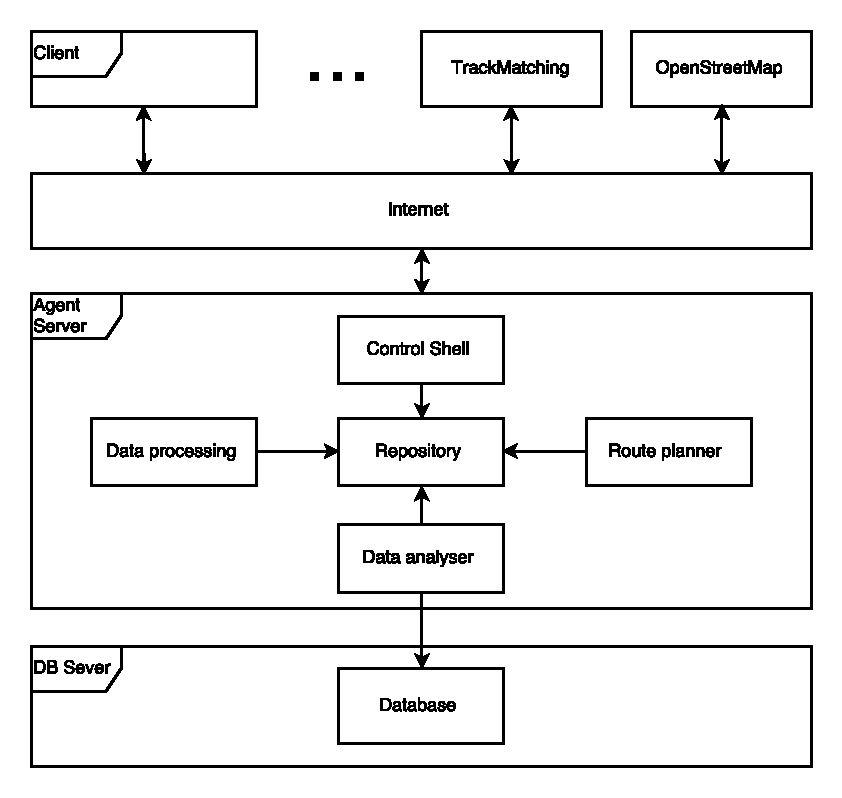
\includegraphics[width=1\textwidth]{figures/architecture.pdf}
    \caption{A course grained system overview.}
    \label{fig:systemoverview}
\end{figure}

The system has been designed as a combination of a client-server and a repository "blackboard" pattern. \figref{fig:systemoverview} shows the overview of the system. The main server module encapsulates most of the processing of the system. The clients represent the GPS-enabled devices that communicates live GPS data through an internet connection to the server, which in turn processes and analyses the data in different subsystems. We use two the external services: TrackMatching to map-match, and OpenStreetMap to obtain map information. They are described in \secref{sec:mapmatching} and Section \secref{sec:mapgeneration}, respectively.

The server architecture is designed as a repository structure, where the solution repository is the shared medium of the subsystems. This architecture is often used when working with artificial intelligence, where the solution is gradually built from different contributing systems, which is why we have chosen this structure of the system.

Initially, the solution repository contains nothing but the problem specification, which is the set of route requests from the clients. The job of the subsystems is to transform the specification into a solution. This is done gradually by invoking the different subsystems to perform operations on the problem specification until a solution can be sent back to the client(s). The control shell module controls which subsystem that should be invoked, based on the contents of the solution repository. 
%The flowchart shows how the user inputs their destination at the start, which sent to a central server together with the source start address. Ther server then uses the data to calculate a route based on the request. The route calculation is based on a initial model of the roadnetwork, such as speedlimits and other restrictions on the roads, and also historical data that have been gathered over time from the users. The route is then sent back to the user, while driving the user will send data back about the drive, this will be the GPS points of the route. This information is then processed and analyzed to check if traffic conditions are as they are supposed to be, and if not the information can be used to recalculate routes for all the drivers which are passing through a that given segment.\todo{review section to describe new architecture}
\section{Knowledge representation}
In this section we describe what we are going to consider knowledge in the system and how we are going to represent that knowledge. More specifically, we consider how we can model knowledge about the road network and traffic in Beijing. We consider the knowledge representation for several reasons. First of all, the raw GPS samples and map data is not really useful to reason about, as there are a lot of unnecessary details included. Thus, we want to make sure that the model adequately portrays the real roads and traffic of Beijing only with the required level of detail. Secondly, we want to be able to reason about this knowledge to later be able to find patterns in the traffic.
% WHAT is going to be in this section
% WHY are we bothering with this section?
% HOW follows from the subsections.

\subsection{Road network representation}\label{sec:road-network-rep}
% Why and what?
To represent the road network, we must model what the road network consists of. A road network generally consists of roads and intersections of roads. Obviously there are many different types of roads, such as bridges, boulevards and one-way roads, which all have different properties related to how you can travel on them. Instead of differentiating between types of roads, we can see them as a single type of road, having attributes with different values. As such, to represent the road network we use a weighted, directed graph.

% How ?
Let G be a weighted directed graph $G(V,E)$, where $V$ is the set of nodes corresponding to intersections, $E$ is the set edges corresponding to road-segments between nodes. Each edge represents the direction of a road from the origin intersection, $n_o$ to the target intersection $n_t$. That is:
\begin{align*}
  e \in E \text{ is a tuple } e=(u, v) \text{ where } u, v \in N
\end{align*}
Furthermore, two-way roads are represented as two edges,
\begin{align*}
  e_1, e_2 \text{ where } e_1 = (u, v) \text{ and } e_2=(v, u)
\end{align*}
Each edge, $e$, also has an associated weight, $weight(e)$ where  $weight: E \times T \times W \rightarrow \mathbb R_+$ is the weight function as defined more precisely in Section \ref{sec:weight-function}. 

Usually, the weight of an edge is used to choose between edges in search algorithms. Similarly, we construct our weight function for this purpose, as described in \ref{patterns:model-trees}\todo{Skal ref til weight function} 

Representing the road network as a graph is sufficient to capture the important attributes of roads and intersections, since the these attributes can be taken account for by adjusting the weight function to represent differences between different types of roads.

\subsection{Traffic representation}\label{KR:traffic}
We must also consider how to represent knowledge about previous traffic in the Road Network. Since traffic changes over time, we consider this a separate model than the model for the road network, as the traffic describes dynamic properties of the road network, whereas model of the road network represents the static properties.

From the Beijing dataset, we can find many useful properties about the traffic. More specifically, we wish to capture the notion of a person observing the state of traffic when driving on a road at a specific time. An example would be, that a driver could observe that the traffic flows at a lower speed than the speed limit on the road to work in the morning. By collecting many of such \emph{observations} of drivers at different times, we build a large set of observations that can be used to reason about how the traffic situation is at certain time periods. To capture these properties, we define a set of \emph{observations} on road segments.

Let an \emph{observation}, $o$, be:
\begin{align*}
o = (t, d, w, s, e)
\end{align*}
where
\begin{align*}
t \in T &\text{ is the time of day} \\
d \in D &\text{ is a date} \\
w \in W &\text{ is the day of the week} \\
s \in \mathbb{R} &\text{ is the speed and}\\
e \in E &\text{ is road segment where the observation was made.}
\end{align*}

From the map-matched dataset, we obtain the set of all observations on the segments in the road network, by constructing a new observation every time a vehicle is driving on the segment. Fortunately, the time of day, segment identifier, date and week of the day can directly be found in the data. The remaining problem is then to estimate the observed speed.

\subsubsection{Estimating observation speed}\label{KR:speed}
% How to estimate speed
Given a segment, $e \in E$ and a sequence of GPS waypoints, $WP=(wp_1,...,wp_i,...,wp_n)$ where $wp_i = (d_i, w_i, t_i, x_i, y_i)$, we construct a new observation, $o_e$, such that:
\begin{align*}
o_e = (t_1, d_1, w_1, S, e)
\end{align*}
where
\begin{align*}
S = median(\{s_1,...,s_i,...,s_{n-1}\})
\end{align*}
and
\begin{align*}
s_i = \frac{dist(wp_i, wp_{i+1})}{t_{i+1} - t_i} \qquad \text{ for } 0 < i < n
\end{align*}

\section{Map generation}
The map generation is based on the opensource map service OpenStreetMap, where it's possible to export a section of the map. In this export the roads, building etc is included. It is then possible to use APIs to extract the information from de export that are needed. To this we use the tool Osmosis, which is a java API which can query the openstreetmap file.
The output from the osmosis tool is a xml like file, which include nodes and ways. Nodes are road intersections and ways 

The map generation is based on the opensource map service OpenStreetMap, but because their webservice only include the possibility to extract small portions of the map.
Therefore we have chosen to use a mirror site, Geofabrik, which holds extract of the whole map and these are updated daily. This makes it possible for us to extract the whole map for China.

\subsection{Format & Pre-processing}
The maps from Geofabrik in encoded in a comprimized format called pbf. To extract the relevant data from this format we are using a tool Osmosis, to query the file for the information that we need, which are the road network.
We have to limit the query space only to Beijing this can be done by using a parameter called bounding-box where it is possible to specify the restricting longitudes and latitudes for north, south, east and west.
Because the map that we have limited still contains information that are not relevant, we have to 
The map is structured in an xml format, where all points of interest are marked as a node, with tags attatched in it which includes key-value pairs about the point.
Ways almost similar structured, but they also contain a nd tag which contains as it value the id of a node related to the way. 

\begin{lstlisting}[style=XML, caption=Node representation]
<node id, version, timestamp, uid, user, changeset, longitude, latitude >
	<tag key, value />
</node>
\end{lstlisting}

\begin{lstlisting}[style=XML, caption=Way representation]
<Way id, version, timestamp, uid, user, changeset >
	<nd ref />
	<tag key, value />
</node>
\end{lstlisting}

\subsection{Generation}
Here we extract the information left in the export, which are ways and nodes. In this step we generate data data structures to be used in our model, from the ways and nodes. 
\section{Client-server communication}
\label{chap:clientserver}
As mentioned in the former section, we will be using a client-server structure.
The reason behind this choice, is to separate the client application from the back end. Without a client server solution we would not be able to collect data from a client, nor be able to communicate between different devices.
Smartphones used by drivers will be acting as clients,
where they need to be able to send information such as location and speed to the server in some given time interval.
The server will handle this information and send it further for analysing, the server will also send updates regarding the route back to the clients.

The server and the client communicates through an interface, on the application layer, of the Internet protocol suite\todo{kan jeg ikke forstå MP}.
The interface allows an application to set up a connection, and read and write strings.

The interface is implemented as a protocol, that is built upon the Java ServerSocket and the Java Socket,
which handles opening a port, accepting a connection, and connecting to such a port, through a TCP connection.
We chose TCP because it is a stream oriented protocol,
which is ideal for transferring a lot of sequential data from one point to another,
such as a large route planned by the system agent, without corrupting data in the transfer.
The other option would have been UDP, which is a message oriented protocol.
UDP is often used for sending messages from one point to many points,
which minimizes the time it takes for a message to be sent and received.
UDP does not remember the sequence of what it is sending, but TCP does, which is prefered in this case.

\begin{figure}[h!]
  \centering
    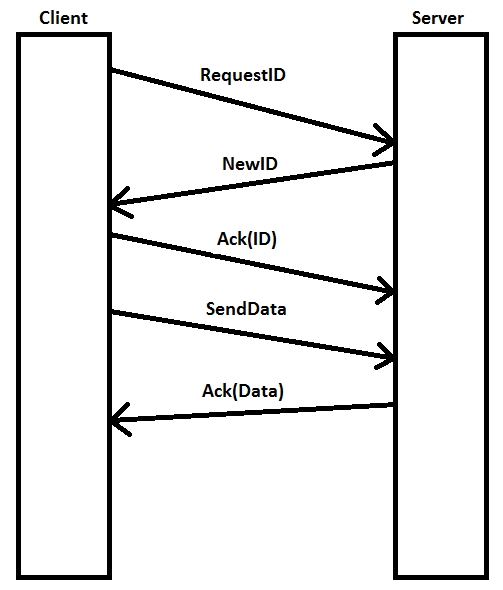
\includegraphics[width=0.4\textwidth]{figures/clientserver.png}
    \caption{Client-server illustration}
    \label{fig:clientserver}
\end{figure}

\figref{fig:clientserver} illustrates how the protocol behave.
The client sends a \textit{REQUEST\_ID} package to the server.
The server responds with a \textit{RETURN\_ID} package,
which contains an integer representing the client ID.
The server picks the ID, based on a local counter, which increases every time a new client connects to the server.
The reason the server provides the ID is to prevent clashes between two client IDs,
which might occur if the clients generated the IDs.
The client sends back an \textit{ACK} package to the server when it has received the ID.
When the client has received the ID, and then acknowledged the ID received,
the client can then send data to the server that is needed to create a new route,
or give information about the route it is following.
The server then sends an acknowledgement that it has received the data.

\begin{table}
\centering
\begin{tabular}{l|p{.6\textwidth}}
\textbf{Type}              & \textbf{Description} \\
\hline
\textit{REQUEST\_ID}       & Package sent to server, requesting a new ID \\
\hline
\textit{RETURN\_ID}        & Response package to a \textit{REQUEST\_ID} \\
\hline
\textit{ACK}               & Sent as acknowledgement that another package was received \\
\hline
\textit{SEND\_DATA}        & Package which includes additional data \\
\hline
\textit{CLOSE\_CONNECTION} & Package sent telling the other side that the connection is closing \\
\hline
\textit{ERROR}             & Error package. Sent when a package could not be processed \\
\end{tabular}
\caption{Types of packages}
\label{tab:package_types}
\end{table}

\tabref{tab:package_types} describes the different types of packages in the protocol.
A package consists of a package header, optionally followed by data.

The messages that are sent back and forth are converted into bytes.
In \figref{fig:bytesclientserver} it is illustrated how the bytes in the package header are packed.
32 bits are reserved for our ClientID, which is empty when the first message is sent to request an ID.
Next we have our RequestID which is a 16 bit integer denoting the ID of the package,
and for identifying the type of package there are 7 bits.
We have reserved one bit as a Last message bit, which is used to be able to tell if a big message,
that is split into 2 or more files has ended.
Lastly there are 8 bits for an integer which is used in case a \textit{SEND\_DATA} request i too large for a single package,
and has to be split into several packages.

\begin{figure}[h!]
  \centering
    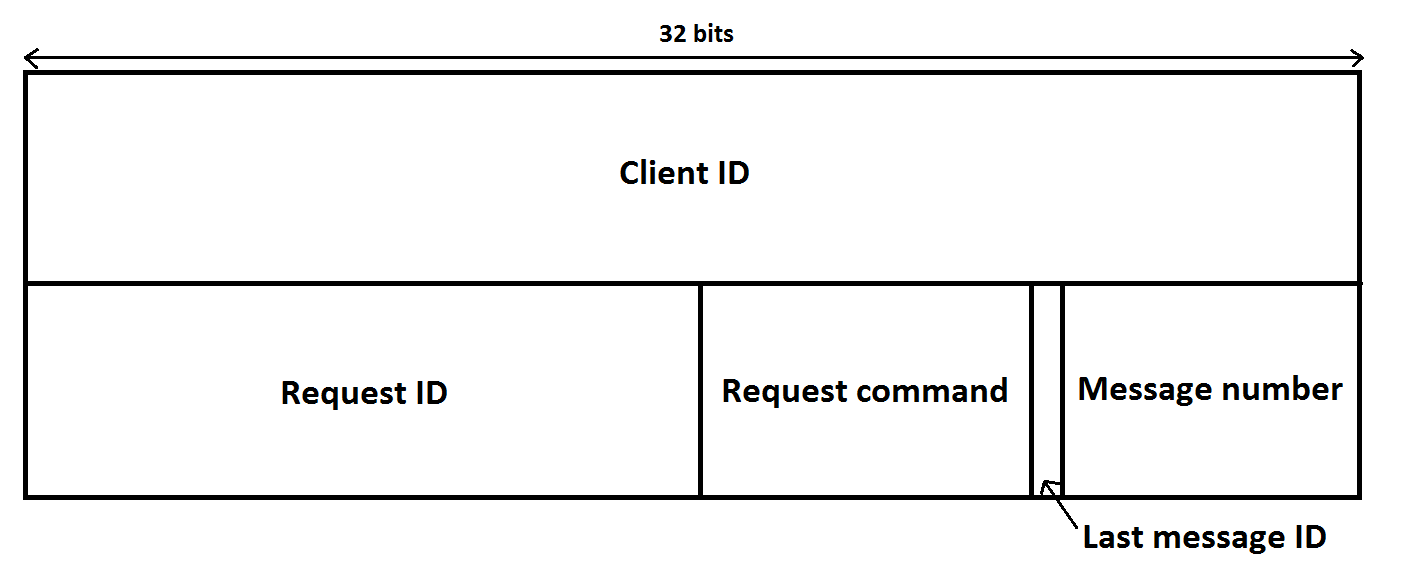
\includegraphics[width=1\textwidth]{figures/bytesclientserver.png}
    \caption{Illustration of header composition}
    \label{fig:bytesclientserver}
\end{figure}\todo{det der vi snakkede om med striberne}

The client updates its GPS location every 5 seconds, so as to be able to maintain a precise location of the client. This information\todo{mangler noget her}, the speed, and the time is sent to the server, and can be used to learn traffic patterns.
%When a message is sent either from the client or the server,
%they are both set to wait for 5 seconds to receive the acknowledgement message, if no such message is received the message is discarded. We could have continued to try and resend the message several times, but a lost GPS coordinate from a user is not a critical problem for our system and will not have any major effect on our calculations.

To be able to show the fastest route a person should drive we have chosen to implement a map on the client. We have implemented an OpenStreetMap viewer and a getRoute method where the client asks for a route between two points, this is done by sending 2 node ids, node ids are explained in \secref{chap:FormatPre-processing}, to the server where then the fastest path is calculated between the 2 points. The server then sends GPS locations of the route which then is shown in the OpenStreetMap on the client. An illustration of this can be seen in \figref{fig:routeonmap}.

\begin{figure}[H]
  \centering
    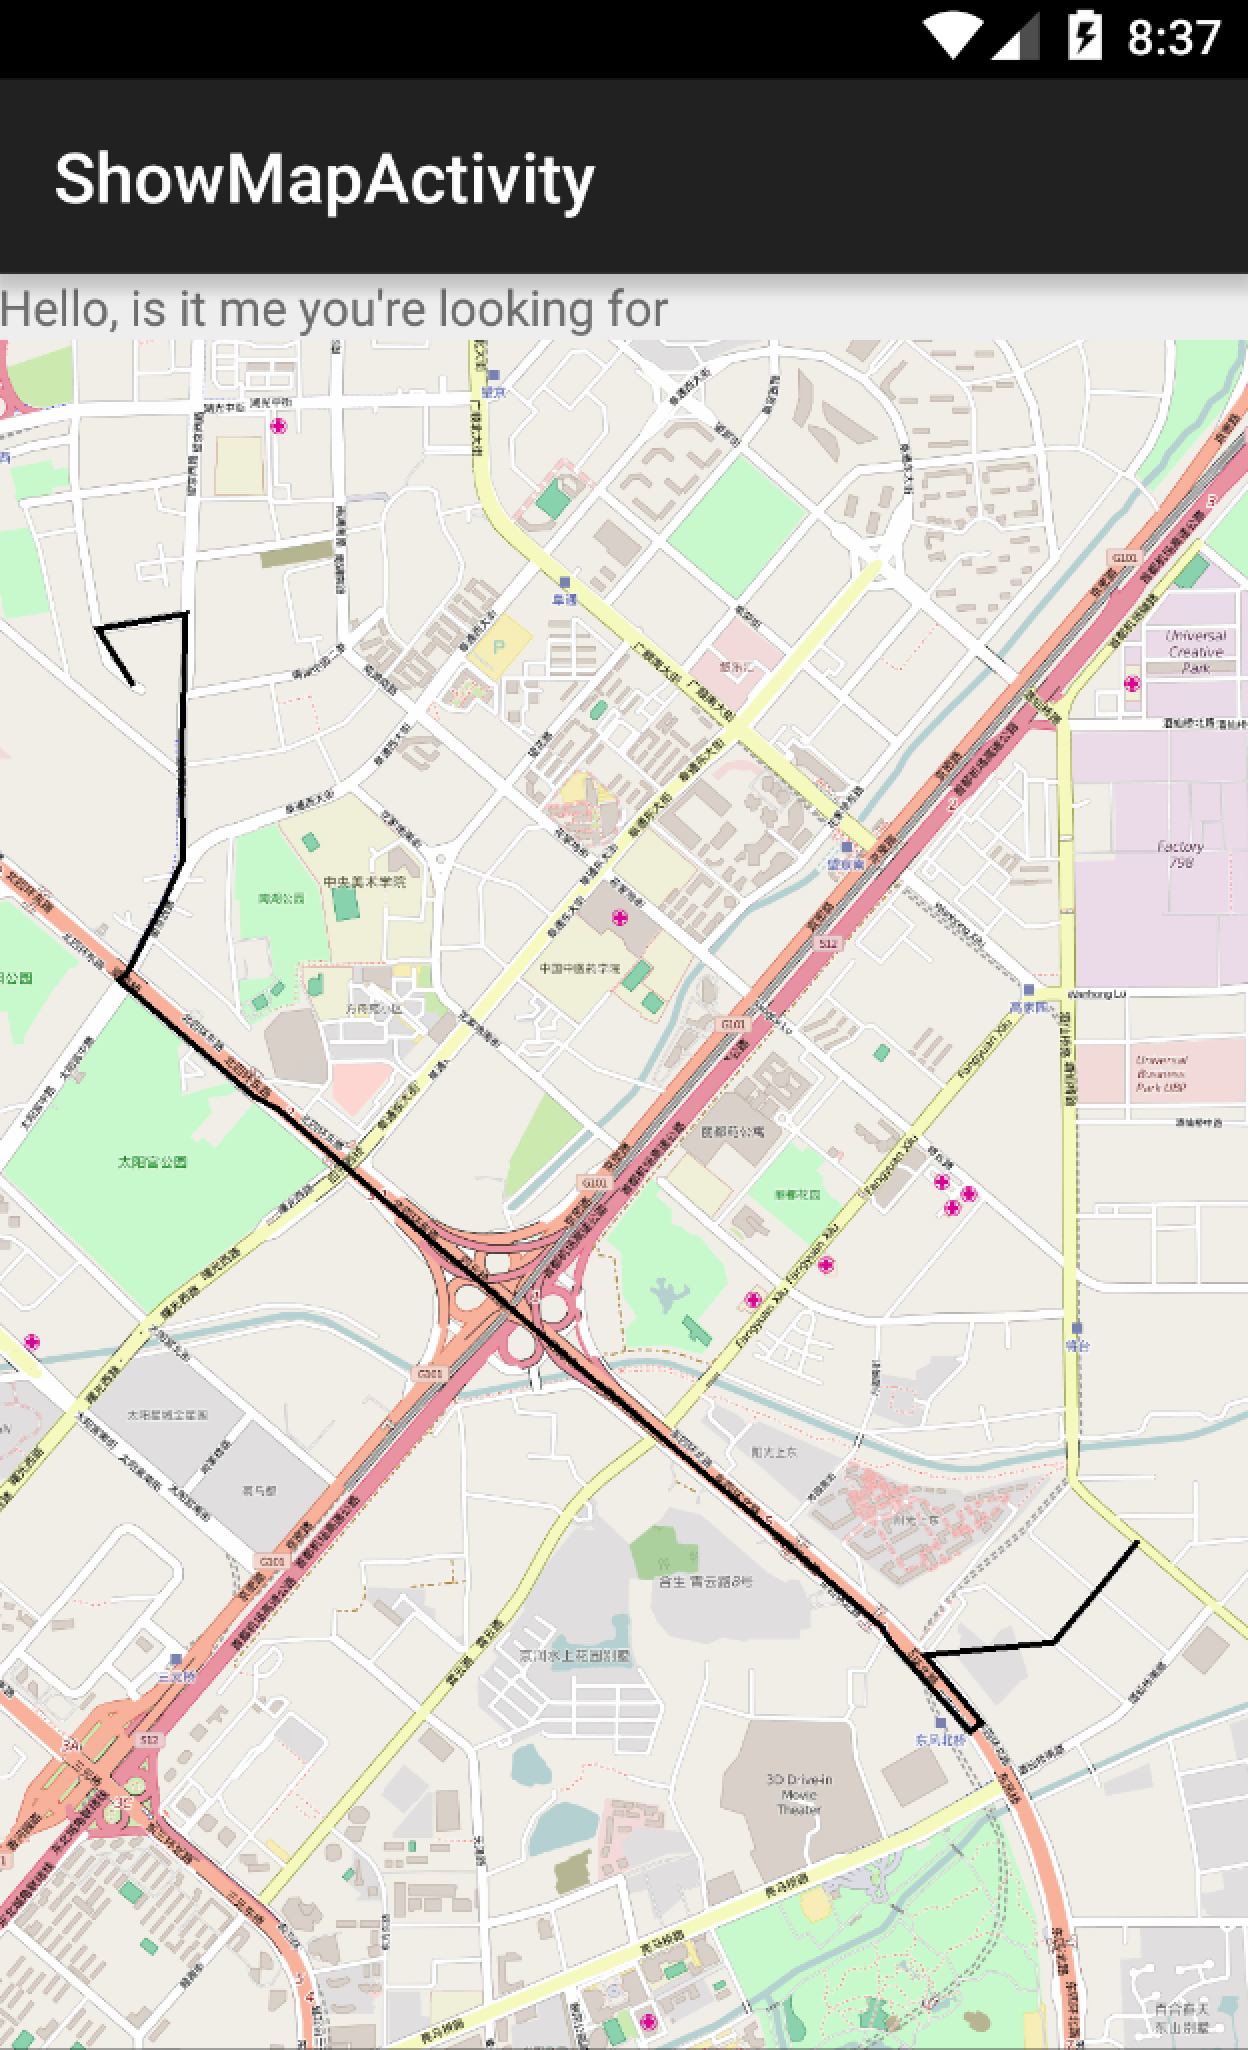
\includegraphics[width=0.6\textwidth]{figures/routeOnMap.png}
    \caption{Illustration of a route sent from the server to the client shown on an android device}
    \label{fig:routeonmap}
\end{figure}

\section{Data Preprocessing}
Here we discuss how to process the Beijing dataset. The overall process is illustrated in \ref{fig:data-processing}. 
\begin{figure}[h!]
  \centering
    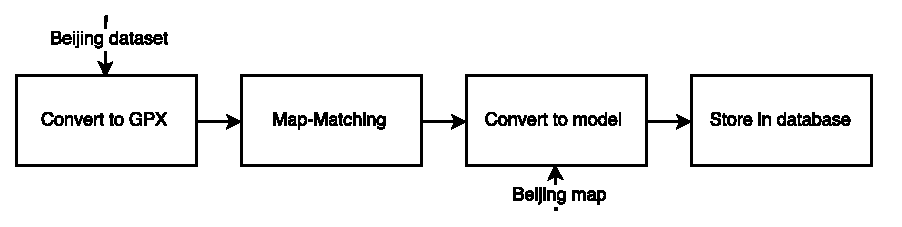
\includegraphics[width=1\textwidth]{figures/data-processing.pdf}
    \caption{From raw gps data to database}
    \label{fig:data-processing}
\end{figure}
The gps dataset is converted into the GPX format which is subsequently map-matched to the road network of Beijing. The map-matched data is then converted into the model objects of the system, and are then stored in the respective tables of the database. Likewise, the map of the Beijing road network is converted to model objects and stored in the database. By doing so, we have a knowledge base of the road network of Beijing and data about vehicle movements in a unified format. \todo{maybe we should perform some data cleaning}
\subsection{Map generation}
To model the road network of Beijing we need to have the specific information about all the roads in the road network. This information is available several places, but most of these services are not free. We have chosen to work with OpenStreetMap which is an open source map service, where users collaborate to keep the city maps updated. There are some problems in using this kind of service, such as the possibility of wrong data, limited data, etc\todo{Er det godt nok bare at skrive etc? + kilde?}. But because this service was the only free service that we could find, we see no other option than having in mind that these problems can occur. We have also found that OpenStreetMap cannot export large areas of a map, such as the whole city of Beijing. Therefore we have chosen to use one of its mirror sites, Geofabrik, which holds extract\todo{Forstår ikke helt det?} of the whole world, segmented into countries and these are updated daily. This makes it possible for us to extract the whole map for China.

\subsubsection{Format \& Pre-processing}
The maps from Geofabrik comes in a compressed format called pbf. To extract the relevant data from this format we are using a tool called Osmosis, to query the file using several filters to be able to extract only the information relevant.
We are using two types of filters with Osmosis, the first is to limit the area that we want to extract, since the map we got is for all of China. The second filter is used to extract only roads from the restricted area.
With this filter we have the possibility to specify which roads we want to have in the output. Because all paths are marked in OpenStreetMap as a way, we want to filter paths such as side-walks, bicycle ways, and other ways that are not possible to use with a car.

The extracted data from the Osmosis query is then exported to a file which is structured in a way that resembles the XML format. There are two types left in the export, which are nodes and ways. Nodes represent road intersections and are also used to indicate points along a road if the road is curved. Both nodes and ways can include key-value pairs that contain information, i.e. if a way is one-way, if a intersection have a traffic light, ect\todo{igen, er etc godt nok at skrive?}.
Ways are almost similar structured, but they also contain a nd tag which contains a value the id of a node related to the way.\todo{Forstår ikke den sidste sætning her}

\begin{lstlisting}[style=XML, caption=Node representation]
<node id, version, timestamp, uid, user, changeset, longitude, latitude >
	<tag key, value />
</node>
\end{lstlisting}

\begin{lstlisting}[style=XML, caption=Way representation]
<Way id, version, timestamp, uid, user, changeset >
	<nd ref />
	<tag key, value />
</way>
\end{lstlisting}

We have illustrated the representation of nodes, ways, edges and segments in \figref{fig:waywithnodes}. Where the red nodes are intersections, the green nodes are points along a way, ways are the black lines, edges are the lines between every node, and a segment is the blue lines between intersection nodes.

\begin{figure}[h!]
  \centering
    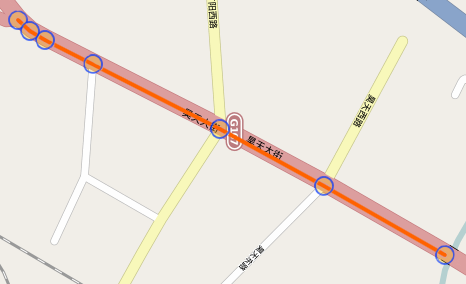
\includegraphics[width=0.8\textwidth]{figures/way-w-nodes.png}
    \caption{A way with nodes}
    \label{fig:waywithnodes}
\end{figure}

\subsubsection{Generation}
To be able to extract the information in the Osmosis export, a XML parser is used to model the road network. When a node or way tag is read a equivalent data structure is created and stored. 
\begin{lstlisting}[style=java, caption=Datastructure for a node]
Node{
	long id;
	double longitude;
	double latitude;
	Ways[] connectedWays;
}
\end{lstlisting}

\begin{lstlisting}[style=java, caption=Datastructure for a way]
Way{
	long id;
	Node[] connectedNodes;
	int type;
}
\end{lstlisting}

We want to model the road network as a graph, but the relation between ways and nodes are not in this format when exported from Osmosis, so we have to work on the data structures generated from the parser.
Besides the original way and node data structures, we have chosen to create two other classes such that we are able to construct a graph, these are called edges and segments.
Edges are the links between every two nodes and a segment is the link between to intersection nodes. When generating these classes from ways and nodes, we have to check whether a way has a tag attached to it which describes if the way is one-way or not, because if it is we have to create edges and segments in both directions.

\begin{lstlisting}[style=java, caption=Datastructure for an edge]
Edge{
	long id;
	double length;
	long origin;
	long destination;
	long segment;
}
\end{lstlisting}

\begin{lstlisting}[style=java, caption=Datastructure for a segment]
Segment{
	long id;
	double length;
	long way;
	long origin;
	long destination;
}
\end{lstlisting}

The relation between edges and segments is that each edge of a segment contains a reference to the segment that it is a part of, the same is true from the relation between ways and segments.
\subsection{GPS sample cleaning}
% WHAT IS IT?
% WHY DO WE DO IT?
% HOW DO WE DO IT?
We perform a simple process of cleaning the GPS data, by filtering GPS samples from outside the physical city limits. The limits are given by a bounding box defined by the coordinates \todo{insert coordinates}. Cleaning the data before further processing is key, since not all of the data is accurate or even useful for reasoning about the traffic. We Even though of the data that is filtered is reliable enough, we delimit our focus on congestion in the city center, so we chose to look aside this data. Since most of the data is clustered in the city center anyway, we do not lose significant parts of the dataset by filtering these samples.\\
Furthermore, some GPS samples are of very bad quality. Some routes are (according to the GPS samples) at one moment driving through Bejing, and the next moment suddenly driving in Africa or Europe. This phenomenon could be caused by weak connection to the GPS satelites e.g. when driving through are tunnel. The inacuraries these corrupt samples introduce, are taken care of as well by filtering samples outside of the city limits. Fortunately, we do not lose all of the samples associated with the rest of the route involved - just the corrupted sample.\\\\
GPS samples that is shown to have completely unrealistic properties is also cleaned from the dataset. An example would be the speed driven between two samples relative to the change in distance between the sampling timestamps. If the speed required to move the physical distance in that time is unrealistic (say, well above what a car can actually drive), we filter these "bad" observations. Note that we actually postpone the filtering of these samples, as it is easier to take into account after mapmatching of the GPS samples has been completed. 

\subsection{Map matching}
The Beijing dataset consists timestamped samples of gps-coordinates. The format of the samples is (id, date time, longitude, latitude). However since GPS measurements can be inaccurate, it is not always possible to directly infer which road the sample was taken on. Consequently the coordinates must be map-matched to a road, such that positions on the road can be inferred. To perform map-matching, the system calls the TrackMatching webservice\cite{TrackMatching}. This service exposes an API for map-matching to the OpenStreetMap service and given a dataset of raw GPS-coordinates returns a map-matched dataset in JSON format. 
\todo{write about how and why map generation}
\todo{write about how and why we design DB and store data in SQL database}
\section{Finding traffic patterns}\label{traffic-patterns}
% Why find traffic patterns?
% What is this section for?
% How? --> follows from the subsections.
In order to reason about the traffic in Beijing, and provide some measure of how the previous traffic possibly affects our belief in how the future traffic situation will be in the road network, we analyse the preprocessed data to look for patterns. In this section, we consider methods for extracting such patterns and propose how to apply them on the Bejing dataset.
\subsection{Methods}\label{patterns:methods}
From our knowledge representation of the road network and traffic, we want to predict how traffic affects the travel time of roads in the road network. In order to do this, we need a measure of the traffic on roads. There are several ways one could construct such a measure, incuding
\begin{itemize}
\item \emph{capacity}: How many vehicles can travel on a road, safely, while not negatively affecting the average speed driven on the road?
\item \emph{classification}: Define a class feature of a road, that defines the state of the road. An example could be $Traffic \in \{free, light, medium, heavy\}$. A given road then has a classification based on the observations of speed within some time period.
\item \emph{speed}: we measure the traffic on a given road, by how fast you can drive on the road. In addition, one could measure the ratio between speed and speed limit.
\end{itemize}
The capacity of a road would be possible to estimate from the speed limit, length of a road, safety distances and number of cars. However, drivers do not always drive in a uniform manner, which makes it difficult to accurately estimate capacities.\par
Performing some discrete classification could help to distinguish between different traffic states. Intuitively, a person might be interested in knowing if a road is clear, mildy congested or heavyily congested. Such information could be captured by classifying roads by a roatio between speed limit and actual speed. This raises the questions of which classes should be used and how many. If there are not enough classes, it might be difficult to choose which road to take if both are congested more or less equally.\par

To more easily be able to evaluate roads where traffic is similar, we must use a measure that has a finer granularity. By looking directly at the actual speed driven on roads, we can determine more precisely the costs of taken a particular road. The actual speed, together with the length of a road is also the most important factors in in evaluating the travel time for a road. Therefore, we take a regression approach for predicting traffic.
\subsection{Regression model}\label{patterns:regression-model}
To predict the traffic speed on a given road segment, at a given time we can consider a speed prediction a function:

\begin{align}\label{eq:speed}
speed: E \times T \times W \rightarrow \mathbb{R}
\end{align}
that maps a road segment, time of day and day of week to the a real valued speed prediction. The remaining question is then, how to actually perform the prediction of traffic on a segment given a specific time. \par
Predicting the numeric value of some variable based on previous observations is typically associated with regression. Regression fits input and output pairs to a function, such that future values for input pairs can be predicted. Fitting a regression function on the observations for a particular road segment, provides a way to predict the traffic on the segment. However, since traffic varies over time, one could argue that a polynomial regression function would fit the observations better than a linear function as illustrated in figure \ref{fig:compare-regression}.
\begin{figure}
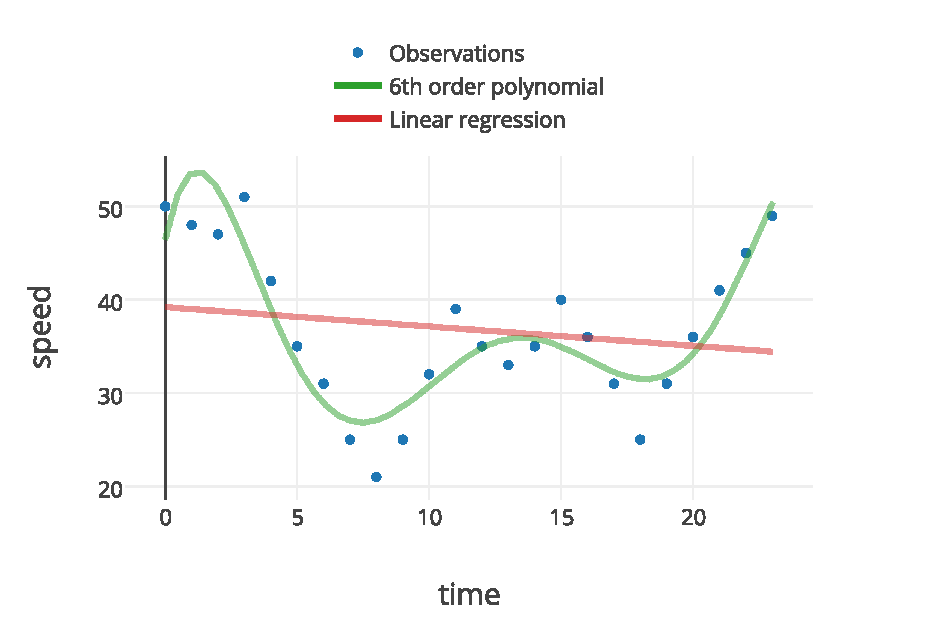
\includegraphics[width=\textwidth]{figures/compare-regression.pdf}
\label{fig:compare-regression}
\caption{Different regression fits on the same dataset.}
\end{figure}
Even though the higher order regression functions generally fits the training data better, such a fit might cause \emph{overfitting} observations, where the accuracy of future predictions decreases and the a linear fit might fit the future observations better. \par
However, a linear regression over the observations for a whole day is not as useful for predicting the fluctuations in traffic during the day, because linear functions by definition cannot model large fluctuations. For this reason, we instead utilise several linear regression models over the course of a day. More specifically, we split a day into partitions $p_1,...,p_i,...,p_n$ where $p_i = (t_1,...,t_j,...,t_k)$ and $t_1,t_2$ are time-stamps. Thus, a partition is defined as a period of time between $t_1$ and $t_2$ that contains every possible timestamp $t_j$ from $t_1$ to $t_k$. For every $p_i$, we perform a linear regression fit, $f_i$, over the observations within that period of time where $f_i:E \rightarrow \mathbb{R}$. In practice, the overall regression function, $speed$, for a road segment becomes a piecewise linear function:
\begin{equation}\label{eq:speed-piecewise}
speed(e,t, w) =
\begin{cases}
f_1(e)       & \quad \text{if } t \in p_1\\
f_2(e)  & \quad \text{if } t \in p_2\\
&\vdots\\
f_n(e) & \quad \text{if } t \in p_n
\end{cases}
\end{equation}

where $f_1,...,f_n$ are linear regression functions for each partition over the observations for segment $e$. The idea is illustrated in Figure \ref{fig:segmented-regression}.
\begin{figure}
\centering
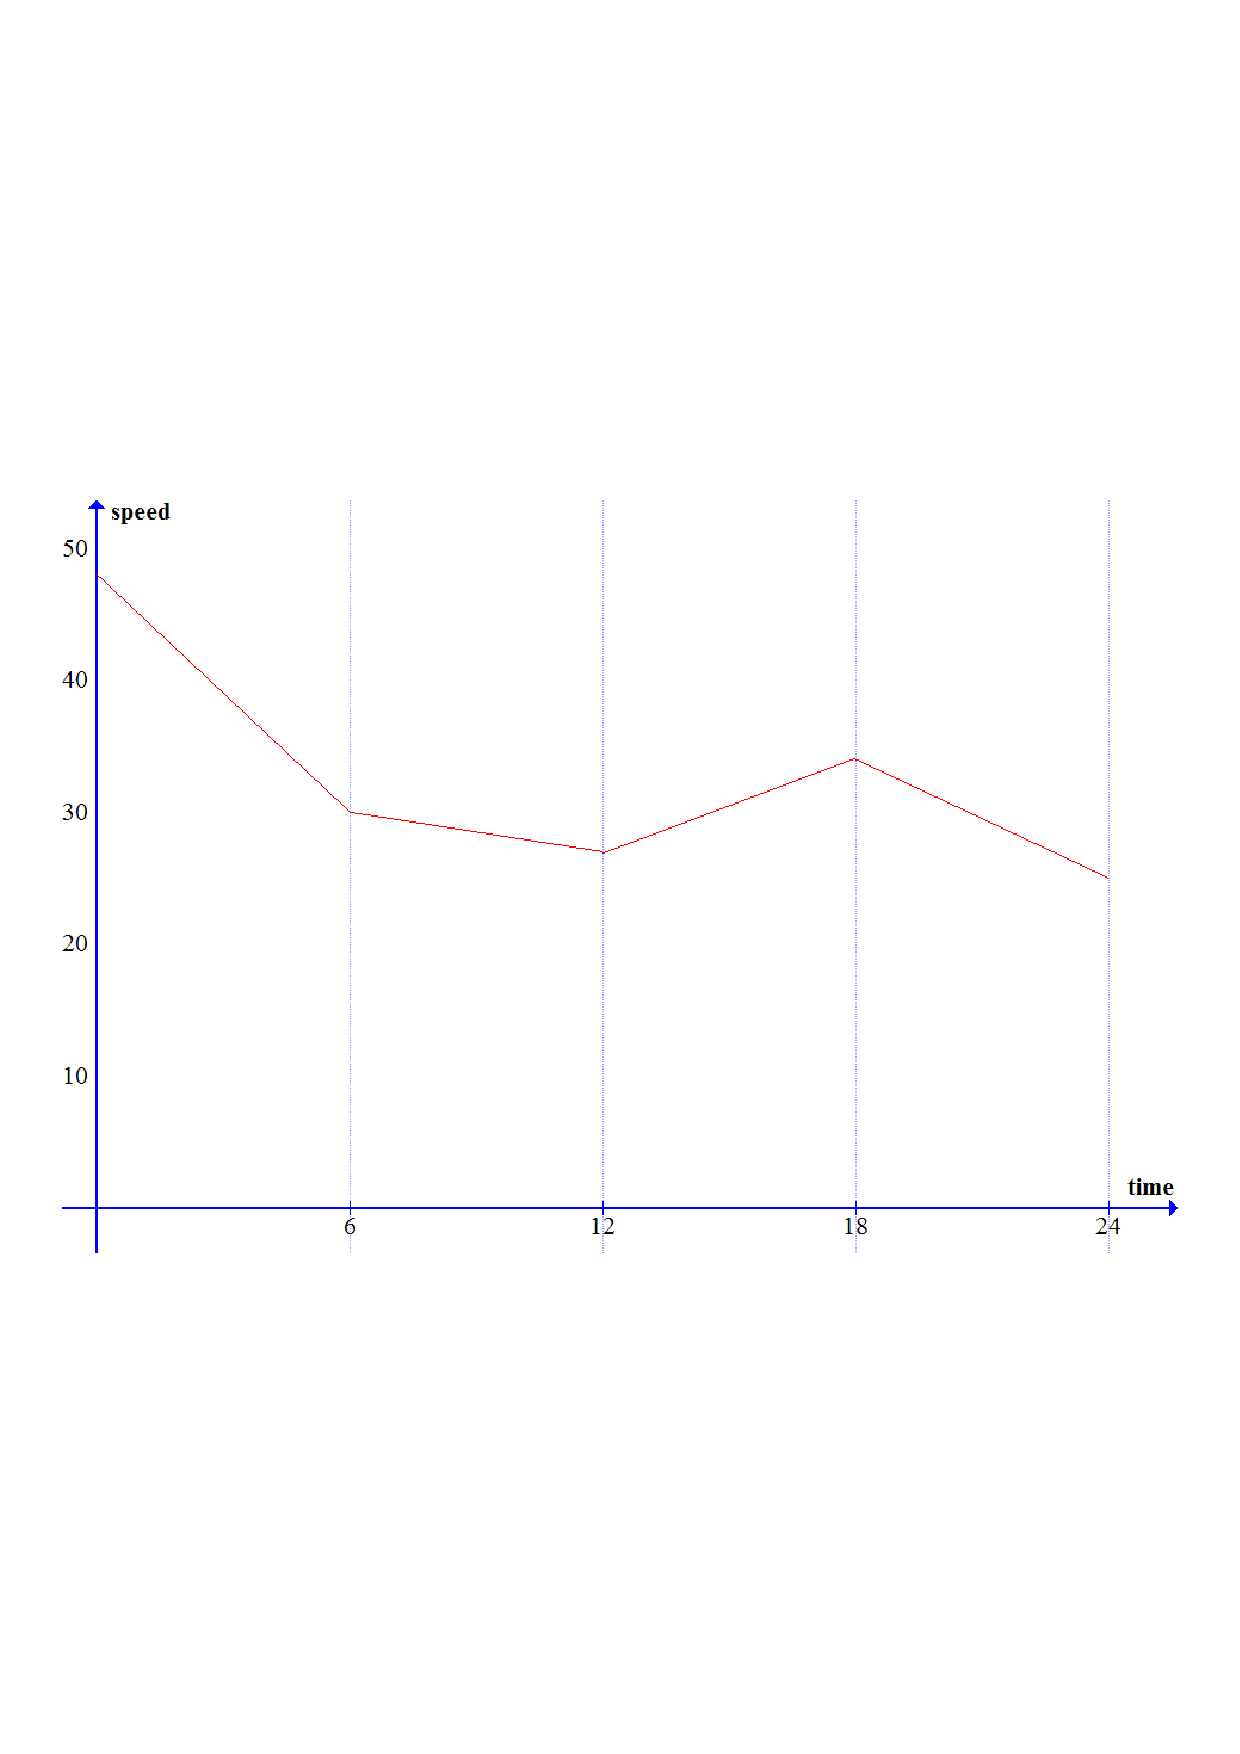
\includegraphics[trim={0 9cm 0 9cm},clip, width=\textwidth]{figures/piecewise.pdf}
\caption{Example of piecewise linear regression - day of 24 hours are partitioned into 4 parts. Every partition has a linear function describing traffic in this time period.}
\label{fig:segmented-regression}
\end{figure}
% Why use it?
% - We want to predict impact of traffic on travel time.
% - How do we measure traffic ?
% 	-	Capacity of roads?
% 		- Difficult to determine accurately, people drive unsafe?
% 	- 	Speeds on roads?
% 	-	Try to classify on congestion?
% 		- k-ary class feature, that classifies a road.
% 		- Penalty of different classes.
% 		- How do we discretize our data into reasonable classes?
% 		- What about roads costs that are almost equal?
% 		- Classes defined by us might not reflect reality.
% 	-	Speed is more "pure" measurement of travel properties of a road
% 		- Speed tells both tells us the penalty of driving on road and has a better granularity of deciding between two almost equal costs of roads.
% 		- Methods for learning traffic:
% 			-	Linear regression
% 			-	Polynomial regression
% 				- Fits the learning data better, but might not fit future samples better! (SSE)
% 			-	But! Traffic also changes over time? (day, week etc..)
% 			-	Divide days into segments, for every segment define fit a linear regression function.
% 			-	How do we segment days?
% 			-	Residual sum
% 			-	Algorithms, M5P automatically splits and generates linear functions
%
% What is it?
% How did we use it?
% Alternatives ?
\\
\subsection{Partitioning scheme}\label{patterns:segmentation}
% Why do it?
%	Want: piecewise linear functions, but how should we partition the days?
In order to use the piecewise linear regression approach, we must devise a partitioning scheme. One such scheme could be the one in Figure \label{fig:segmented-regression} where every day a split into 4 equal partitions: night, morning, afternoon, evening. The following problems are raised by the choice of partitioning scheme:
\begin{itemize}
	\item Where should we split the day, such that important changes in traffic are captured?
	\item How many observations is required to perform regression?
	\item How do we guarantee enough observations in every partition?
\end{itemize}
While it makes sense to have equally sized partitions, it does not guarantee that there will be enough observations to perform a accurate regression for every partition (an example would be, that there are usually less vehicles driving at night, thus less observations in this partition). Furthermore, since traffic patterns most likely are different for different road segments, a static partitioning is not guaranteed to capture important patterns in traffic, such as morning traffic. Therefore, we must incorporate a finer granularity in the partitioning scheme, possibly different for every segment, to capture the differences traffic patterns and to ensure that there will be enough observations to actually perform regression.

This leads us to a dynamic partitioning scheme, where the partitioning is based on the density of observations and how well the function fits the data. A measure to use for such a partitioning, could be the Sum of Squared Errors, which is a measure of how close a predicted value is to the real value. Partitioning is then done, based on minimizing the Sum of Squared Errors, as this yields more accurate regression models.

%\subsection{Quality measure}\label{quality-measure}
%Some of the observations might be based on a small number of GPS samples, or data that is map-matched with a high error rate (accuracy of which road was best to map-match on). Such observations could potentially introduce noise into the regression model and must therefore be taken into account when we construct the model trees. 

%Furthermore, we are interested in weighing the most accurate data higher than data with worse quality, since more accurate data tells us more about the traffic on a given segment. To do that, we introduce a quality measure of observations. The quality measure describes the ratio between the number of GPS samples used to create an observations, and the length of the road segment where the observation was made. That is, the quality measure, $Q$ of an observation, $o$ is given by:
%\begin{equation}
%Q(o) = \frac{|wp|}{|e|}+0.29
%\end{equation}
%where $|e|$ is the length of a road segment $e$, and $|wp|$ is the number of waypoints used to construct $o$.
% Why?
% 	some data might be unreliable, better to use good data first
% What?
% 	We introduce a quality measure --> such that we can decide which observations are "better" in the sense of accuracy observations.
% How?
%	based on the ratio between the length of the segment and the
%	number 	of 	waypoints
% Could also include error rate from mapmatching, but unsure what it means (probably means accuracy of which the mapmatching was done)

\subsection{Model trees}\label{patterns:weka}
% What is it? (M5P algorithm)
% Why use it? (does exactly what we need)
% How do we use it? (M5p in weka)
For implementing regression models and data filters, we use the machine learning tools and algorithm implementations in Weka. Weka can be invoked directly from Java code, and therefore integrates well with our system.

The piecewise linear regression model described in Section \ref{patterns:regression-model} is implemented using the the M5P tree induction algorithm. M5P is an implementation of the M5' algorithm\cite{IMTCC96}. M5P constructs a model tree, like the one illustrated in Figure \ref{fig:model-tree}, from a set $T$ of training examples, with regression models at the leaves that are either functions or constants.

\begin{figure}[H]
	\centering
	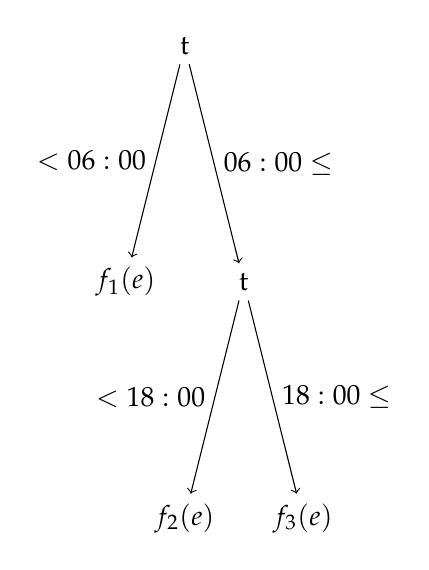
\begin{tikzpicture}
	\node {t}
	[level distance=3cm]
	child { node {$f_1(e)$} edge from parent [->] node [left] {$ < 06:00 $} }
	child { node {t}
		child { node {$f_2(e)$} edge from parent [->] node [left] {$ < 18:00 $}}
		child { node {$f_3(e)$} edge from parent [->] node [right] {$ 18:00 \le $} }
		edge from parent [->] node [right] {$06:00 \le $}
	}
	;
	\end{tikzpicture}
	\caption{Example of a simple model tree with three partitions and three linear regression models. The $t$ feature corresponds to the input time feature in equation \ref{eq:speed-piecewise}}
	\label{fig:model-tree}
\end{figure}

It works by recursively constructing a decision tree by splitting $T$ into subsets $T_1,T_2$ where the split point is determined by:\todo{Morten Trello: Fix}
\begin{enumerate}
\item Choosing the attribute $A$ that contains the best split.
\item Choosing the split in $A$ that yields the highest reduction in standard deviation.
\end{enumerate}
The resulting tree is then pruned for nodes and leaves that yield a worse standard deviation reduction than parent nodes. This pruning makes sure the final model is not overfitting the training examples and can better be applied to unknown data. 

Finally, the resulting regression models at the leaves of the tree are mutually smoothed as to avoid having sharp transitions from model to model.
Using this approach, the algorithm facilitates a dynamic partitioning scheme, based on the measure of standard deviation. 

\subsubsection{Data filtering}
Some of the observations might have been matched to the wrong road, based on a small number of GPS samples, etc. Such observations could potentially introduce noise into the regression model and must therefore be taken into account when we construct the model trees. To accomplish this we utilise a few filters for preprocessing the observations. Only speeds below two times the speed limit are used. The remaining speeds that exceed the speed limit are lowered to the speed limit so as to not encourage speeding. Additional filters can be seen in \tabref{tab:datafiltering} (the green row is the one we use), where \emph{MSR} is the median sample rate calculated using only waypoints that are at least 1.4 metres apart, \emph{\#Wpts} is the total number of waypoints on the link, \emph{Length} is the distance driven between the first and the last waypoint in the link, and \emph{Observations} is the number of observations remaining after applying the filters.\todo{Revise when we have decided exactly which filters to use.}

%  SELECT COUNT(o.*) FROM Observations o, Segments s, Ways w, Roadtypes t WHERE o.speed > 1 AND o.speed < t.speedlimit * 2 AND o.length > 0.005 AND o.mediansamplerate <= 20 AND o.error < 100 AND numwaypoints > 4 AND o.segment = s.id AND s.way = w.id AND w.type = t.id;
\begin{table}[H]
	\centering
	\begin{tabular}{TlTlTlTlTlTlT}
		\thickhline
		\textbf{Speed}                                                                          & \textbf{Length}  & \textbf{MSR}  & \textbf{Error} & \textbf{\#Wpts} & \textbf{Observations} \\ \thickhline
		-                                                                                       & -                & -             & -              & -               & 4584306               \\ \thickhline
		\begin{tabular}[c]{@{}l@{}}\textgreater 1 km/h\\ \textless speed limit * 2\end{tabular} & \textgreater 5 m & \textless= 20 & \textless 100  & \textgreater= 5 & 269527                \\ \thickhline
		\begin{tabular}[c]{@{}l@{}}\textgreater 1 km/h\\ \textless speed limit * 2\end{tabular} & \textgreater 5 m & \textless= 20 & \textless 100  & -               & 867128                \\ \thickhline
		\begin{tabular}[c]{@{}l@{}}\textgreater 1 km/h\\ \textless speed limit * 2\end{tabular} & -                & \textless= 20 & \textless 100  & -               & 878426                \\ \thickhline
		\textless speed limit * 2                                                               & -                & \textless= 20 & \textless 100  & -               & 898774                \\ \thickhline
		\textless= speed limit                                                                  & -                & \textless= 20 & \textless 100  & -               & 861766                \\ \thickhline
		\textless= speed limit                                                                  & -                & \textless 300 & \textless 100  & -               & 2861949               \\ \thickhline
		\rowcolor[HTML]{34FF34}
		\begin{tabular}[c]{@{}l@{}}\textgreater 1 km/h\\ \textless speed limit * 2\end{tabular} & \textgreater 5m  & \textless= 60 & \textless 100  & -               & 1715070               \\ \thickhline
		\begin{tabular}[c]{@{}l@{}}\textgreater 1 km/h\\ \textless speed limit * 2\end{tabular} & \textgreater 5m  & \textless= 60 & \textless 100  & \textgreater= 3 & 913779                \\ \thickhline
	\end{tabular}
	\caption{Observations remaining after using various filters. MSR = median sample rate of the link, \#Wpts = number of waypoints in the link.}
	\label{tab:datafiltering}
\end{table}

Additionally, we perform normalisation of the timestamps of observations, due to Weka3's internal representation of time being problematic when doing regression.

\subsection{Weight function}\label{sec:weight-function}
As mentioned in Section \ref{}, we are interested in calculating how fast one can travel along the road segment (i.e. the travel time), given a road a road segment, time and day of the week. With the regression model for predicting speed on a road segment from time and day of the week, we can compute a prediction for the travel time. Let 
\begin{align}
weight: E \times T \times W \rightarrow \mathbb{R_+}
\end{align}
be the \emph{weight function} that maps an edge $e$, timestamp $t$, and day of the week $w$, to a positive, real-valued travel time.

The weight function works, by calculating the $speed$ function described in Equation \ref{eq:speed-piecewise} and dividing the predicted speed by the length of the given road segment. That is, given $e \in E$, $t \in T$, $w \in W$:
\begin{align}
weight(e,t,w) = \frac{speed(e,t,w)}{len(e)}
\end{align}
where:
\begin{align}
len:E \rightarrow \mathbb{R_+}
\end{align}
is a length function, that maps edges to their length.
\section{Route planning}
In order to be able to suggest routes to motorists, the system must find the best route available at a given time and day of the week. One could define several quality measures of a good route, but in this case we consider the best route in terms of time, that is, the shortest travel time. The process is known as finding shortest paths in a directed weighted graph, and existing algorithms solve this problem well. In this section we discuss the methods used for finding such shortest paths.

\subsection{A* Heuristic Search}\label{sec:pathfinding}
We use the heuristic search algorithm A* since it is a widely used approach for finding shortest path routes in graphs and can be improved by further preprocessing of the graph as discussed in \chapref{ch:future-work}.

We design the heuristic as an underestimate of the real travel time from a given node to the target node, by letting the heuristic be the travel time of traveling the Euclidean distance at 120 km/h (i.e. the highest speed limit in Beijing) from a given node to the target node.

Let $h(v)$ be the heuristic function:
\begin{align*}
h(v) = &\frac{dist(u,v)}{120 km/h} \qquad u,v \in V
\end{align*}
that computes an underestimate of the travel time from $u$ to $v$ to ensure the graph search proceeds in the correct direction in the graph.

At every expansion of a node, each of the weights of the neighbouring nodes are computed using the weight of the segment that leads from the node being expanded to the neighbour at a particular time of a given day. Each time a node is explored the weight of the current node added to the start time will be used as the time when calculating the weight of each of the neighbouring nodes. The idea is illustrated in \figref{fig:timed-graph}.

\begin{figure}[h]
\centering
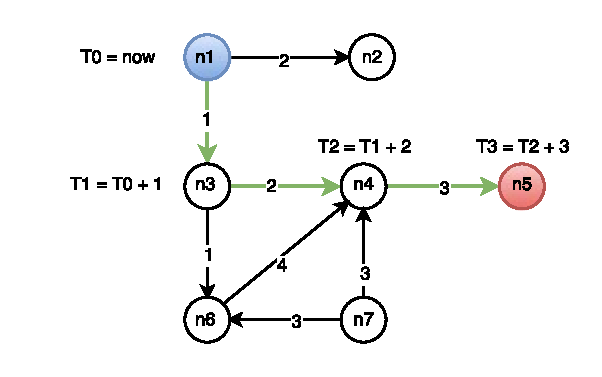
\includegraphics[width=\linewidth]{figures/timed-graph}
\caption{Relative times in path-finding - Numbers on edges are weights in time. Relative time is indicated next to nodes. The green arrows indicate the shortest path found. The weight of each segment is calculated based on the time of the origin node.}
\label{fig:timed-graph}
\end{figure}

%An A* is used to finding a path through the graph. There are other versions of a A* search that are faster then a normal A*, but these do not work with the weight function that are being used. The time complexity of this search is $O(b^n)$ where $b$ is the branching factor and $n$ is the number of nodes in the graph.

%The function is given a start and a goal node, the A* utilise the physical destined between these point as a heuristic to make sure the path it takes goes in the right direction. Then it finds the time and ask the database for the cost of the segments it can travel from the node it's at.

%The reason for using this algorithm over other graph search is that the the time for finding a path is $O(b^{(n/2)})$ where a normal Dijkstra’s takes $O(b^{n})$, where $b$ is the branching factor and $n$ is the number of nodes in the direct graph. Bi-directional also have the benefit of working well when running in paralleled.


% How do we use it?
%By using bi-directional search there is one problem that needs to be address, this is will the search meet op before the whole graph is search. There are more then one way of solving this problem, in this project A* have been chosen for solving this problem. The A* makes sure that the search from the start node wakes a path towards the end node and the other way around for the search that starts from end node.

%By implementing the bi-directional search this way, the worst case running time becomes $O(b^{n})$. The reason for this is that each search is going towards the other search's start node and not it's frontier. The search will stop if one of the two searches hits a node that the other search have visited.

\subsection{Weight function}\label{sec:weight-function}
The weight of road segments is the travel time required to travel along a road segment at a specific time and day of the week. With the regression model for predicting speed on a road segment based on the time and day of the week, we can compute a prediction for the travel time.

Let
\begin{align}
weight: E \times T \times W \rightarrow \mathbb{R_+}
\end{align}
be the \emph{weight function} that maps an edge $e$, timestamp $t$, and day of the week $w$, to a positive, real-valued travel time.

The weight function works, by calculating the $speed$ function described in Equation \ref{eq:speed-piecewise} and dividing the length of the given road segment by the predicted speed. That is, given $e \in E$, $t \in T$, $w \in W$:
\begin{align}
weight(e,t,w) = \frac{len(e)}{speed(e,t,w)}
\end{align}
where:
\begin{align}
len:E \rightarrow \mathbb{R_+}
\end{align}
is a length function, that maps edges to their length.

\chapter{Test}
\chapter{Conclusion}
This project presented an approach for modeling road network and traffic as weighted directed graphs with weight functions as time-based piecewise linear regression models over traffic observations of speed derived from GPS samples.

The piecewise linear regression models was found to have an average predictive accuracy of NUMBER\% of actual observed travel time on routes. This follows from several issues still present in the regression models such as limited data and improvable filtering, and could futher be improved by gathering a more useful dataset where speed is directly measured.

Furthermore the system was found to, in certain cases, be able to find alternative routes avoiding traffic congestion thus potentially provide time-savings for users of the system. By providing such a feature the system can help motorists avoid heavy traffic and be more evenly distributed on the road network.

There are many interesting areas for future work including gathering better GPS data, more accurate map-matching , optimizations in terms of utilizing advanced graph methods such as contraction hierarchies to speed up query time. Furthermore, we find it important to perform field-testing in the future, to get a much better perspective of the accuracy of the system as a whole.

To be able to collect the data needed to predict traffic patterns which our agent needs, we have constructed a client-server architecture, which is described in \secref{chap:clientserver}. The client collects data, speed, time and GPS locations, and sends that to our server where we can store the information.
\printbibliography[heading=bibintoc]
\label{bib:mybiblio}
\appendix
\chapter{Routefinding pseudocode}\label{ch:astar}
\begin{algorithm}
\begin{algorithmic}[1]
\Function{A*}{$Graph$, $Start$, $End$}
  \State create vertex set $Q$ \Comment{Set of unvisited nodes}
  \State
  \ForAll{vertex $v$ \In $Graph$} \Comment{Initialization}
    \State $dist[v] \gets$ INFINITY \Comment{Unknown distance from $Start$}
    \State \Comment{to $v$}
    \State
    \State $heur[v] \gets$ \Call{H}{$v$, $End$} \Comment{Heuristic value from $v$ to $End$}
    \State
    \State $prev[v] \gets$ UNDEFINED \Comment{Previous node in the optimal}
    \State \Comment{path from $Start$}
    \State
    \State add $v$ to $Q$ \Comment{All nodes are initially unvisited}
  \EndFor
  \State
  \State $dist[Start] \gets 0$
  \State
  \While{$Q$ is not empty \AND \Call{OtherDirectionNotDone}{}}
    \State $u \gets$ vertex \In $Q$ with min $dist[u] + heur[u]$
    \State remove $u$ from $Q$
    \State \Call{VisitFromThisDirection}{$u$}
    \State
    \If{$u = End$ \Or \Call{IsVisitedFromOtherDirection}{$u$}}
      \State for this direction: $done \gets$ \True
      \State \Return \Call{ReconstructPath}{$prev$}
    \EndIf
    \State
    \ForAll{neighbours $v$ of $u$} \Comment{where $v$ is still in $Q$}
      \State $alt \gets dist[u]$
      \If{$alt < dist[v]$}
        \State $dist[v] \gets alt$
        \State $prev[v] \gets u$
      \EndIf
    \EndFor
  \EndWhile
  \State \Return empty
\EndFunction
\end{algorithmic}
\caption{A* ready for bidirectional search}
\label{alg:bi_astar}
\end{algorithm}

\begin{algorithm}
\begin{algorithmic}[1]
\Function{BidirectionalSearch}{$Graph$, $Start$, $End$}
  \State $path1 \gets$ run \Call{A*}{$Graph$, $Start$, $End$} concurrent
  \State $path2 \gets$ run \Call{A*}{$Graph$, $End$, $Start$} concurrent
  \State
  \If{$path1 =$ empty}
    \State \Return $path2$
  \Else
    \State \Return $path1$
  \EndIf
\EndFunction
\end{algorithmic}
\caption{Bidirectional search}
\label{alg:bi_search}
\end{algorithm}

\end{document}